\chapter{Experimentos e Resultados}\label{cap:resultados}
Esta seção apresenta os resultados das cinco arquiteturas analisadas.
Em seguida, a arquitetura com melhor desempenho é analisada mais detalhadamente sob diferentes aspectos.
Toda a pesquisa foi realizada em uma máquina com placa gráfica NVIDIA GeForce RTX 3060 Ti, processador Intel Core i7-11700K de 3,60 GHz e 16 GB de memória RAM.
% ----------------------------------------------------------
\section{Resultados dos Modelos}\label{sec:modelsresults}

A Tabela \ref{tab:metrics} exibe a acurácia de cada modelo com diferentes taxas de aprendizagem, utilizando o \acrshort{sgd} como otimizador.
A taxa de aprendizagem de 1x10$^{-5}$ apresentou as melhores acurácias no geral, porém não gerou o melhor modelo.
Nenhum modelo obteve boa acurácia com essa taxa de aprendizagem, indicando que um valor muito baixo limitou a capacidade dos modelos de convergir para uma solução satisfatória.

O \textit{MobileNetV2} obteve os piores resultados nas outras duas taxas de aprendizagem avaliadas.
Já o \acrshort{vit} apresentou o melhor desempenho, com acurácia superior tanto para a taxa de aprendizagem de 1x10$^{-3}$ quanto para a de 1x10$^{-4}$.

\begin{table}[tb]
\caption{\label{tab:metrics} Acurácia dos cinco modelos com diferentes taxas de aprendizagem.}
\begin{center}
\begin{tabular}{c|ccc}
\toprule
\multirow{2}{*}{Modelos} & \multicolumn{3}{c}{Taxa de aprendizagem}   \\
                         & 1x10-03     & 1x10-04     & 1x10-05     \\
\midrule
VGG19                    & 0,808 & 0,732 & 0,524 \\
\midrule
InceptionV3              & 0,795     & 0,731     & 0,529        \\
\midrule
DenseNet                 & 0,802     & 0,658     & 0,592     \\
\midrule
MobileNetV2              & 0,781  & 0,608 & 0,534 \\
\midrule
ViT                      & 0,816     & \textbf{0,826}     & 0,511     \\
\bottomrule
\end{tabular}
\end{center}

\end{table}

O desempenho inferior do \textit{MobileNetV2} pode ser explicado por sua arquitetura, projetada para uso em dispositivos com menor poder computacional \cite{mobilenetv2}, possuindo, portanto, um número significativamente menor de parâmetros treináveis em comparação com as demais arquiteturas avaliadas.

Um comportamento comum a todos os modelos, exceto o \acrshort{vit}, foi a redução da acurácia conforme a diminuição da taxa de aprendizagem.
Isso sugere que taxas de aprendizagem muito baixas podem ser inadequadas para ajustar a grande quantidade de parâmetros presentes em redes profundas.

Apesar de tanto o \acrshort{vgg} quanto o \textit{DenseNet} terem alcançado acurácias próximas a 80\%, o \acrshort{vit} apresentou resultados ligeiramente superiores.
Outro aspecto relevante a ser considerado é que, enquanto o \textit{InceptionV3} levou 47 minutos para completar seu treinamento, o \acrshort{vit} realizou o mesmo em apenas 22 minutos no mesmo conjunto de dados.
Portanto, o \acrshort{vit} utilizando taxa de aprendizado de 1x10$^{-4}$ foi selecionado como o modelo a ser utilizado para as etapas subsequentes deste trabalho.
% ----------------------------------------------------------

\section{Avaliação do melhor modelo}\label{sec:bestmodel}

Após a escolha da arquitetura de melhor desempenho e da taxa de aprendizado adequada, outras análises devem ser feitas para saber se é possível melhorar seus resultados e o quão adequado foi seu treinamento.

% -----------------------

\subsection{Validação cruzada K-Fold}

A primeira análise realizada exclusivamente com o \acrshort{vit} foi a aplicação de validação cruzada do tipo K-Fold, utilizando o mesmo conjunto de dados.
A Tabela \ref{tab:kfold} apresenta as métricas de acurácia, precisão e revocação obtidas nos cinco subconjuntos, ou \textit{folds}, empregados na validação.

A acurácia média de 0,801 obtida na validação cruzada foi inferior à acurácia de 0,826 observada na validação simples.
Esse resultado sugere que o conjunto de treino inicialmente utilizado pode ter incluído imagens mais facilmente classificáveis, o que beneficiou o desempenho na validação simples.

Ao analisar cada subconjunto individualmente, observa-se que os folds 2 e 5 apresentaram acurácias significativamente menores em relação aos demais.
Tal comportamento indica que as características das câmeras incluídas nesses subconjuntos de validação não foram adequadamente aprendidas pelo modelo, que foi treinado com imagens provenientes das outras câmeras.
Além disso, a baixa revocação observada no subconjunto 5 pode indicar que o modelo adotou uma estratégia conservadora, prevendo a classe de normalidade apenas em situações de classificação com maior confiança, ao custo do aumento de falsos negativos.

Embora o modelo tenha mantido uma acurácia média aceitável, o desempenho inferior nos subconjuntos 2 e 5 evidencia uma sensibilidade dos resultados à composição das câmeras no conjunto de treino, ressaltando a importância de uma seleção equilibrada das câmeras para garantir generalização adequada do modelo.
% \usepackage{graphicx}
\begin{table}[tb]
\caption{\label{tab:kfold} Métricas do ViT com validação cruzada K-Fold com K=5.}
% \resizebox{\columnwidth}{!}{%
\begin{center}
\begin{tabular}{c|ccc}
\toprule
Subconjunto  & Acurácia & Precisão & Revocação \\
\midrule
1     & 0,833    & 0,838    & 0,827     \\
\midrule
2     & 0,777    & 0,773    & 0,785     \\
\midrule
3     & 0,794    & 0,780    & 0,820     \\
\midrule
4     & 0,819    & 0,801    & 0,849     \\
\midrule
5     & 0,771    & 0,816    & 0,700     \\
\midrule
Média & 0,794    & 0,801    & 0,820     \\
\bottomrule
\end{tabular}%
\end{center}
%}
\end{table}

% -----------------------

\subsection{Métricas no conjunto de teste}

Após a validação cruzada, o modelo também foi avaliado no conjunto de teste, o qual apresenta balanceamento entre as classes, porém não possui balanceamento na quantidade de imagens provenientes de cada câmera que compõe esse conjunto.

A Tabela \ref{tab:test} exibe os resultados obtidos pelo modelo no conjunto de teste, juntamente com seus resultados na validação cruzada.
Observa-se uma leve queda na acurácia, contudo o modelo mantém uma capacidade razoável de classificação.
O aumento na precisão indica que o modelo cometeu menos falsos positivos no conjunto de teste, evidenciando uma classificação mais conservadora da classe positiva.

Entretanto, houve uma queda significativa na revocação no conjunto de teste.
Dessa forma, apesar da postura conservadora, o modelo falhou em classificar corretamente uma quantidade expressiva de verdadeiros positivos.

\begin{table}[tb]
\caption{\label{tab:test} Métricas do ViT no conjunto de teste.}
\begin{center}
\begin{tabular}{c|ccc}
\toprule
Conjunto          & Acurácia & Precisão & Revocação \\
\midrule
Validação Cruzada & 0,794    & 0,801    & 0,820     \\
\midrule
Teste             & 0,780    & 0,814    & 0,719     \\
\bottomrule
\end{tabular}%
\end{center}
\end{table}
% -----------------------

\subsection{Diminuição da intensidade luminosa}
Após a escolha da arquitetura de melhor desempenho, diferentes valores para o fator denominado nesta dissertação como fator de claridade (\textit{FC}), conforme mencionado na Seção \ref{subsec:datapreprocessing}, foram avaliados utilizando o \acrshort{vit}, com o objetivo de analisar se o modelo poderia ser aprimorado ao levar em consideração a claridade excessiva presente em algumas imagens.

A Tabela \ref{tab:brightnessfactor} apresenta o desempenho do \acrshort{vit} com quatro valores distintos para o \textit{FC}, sendo que o valor 1 para o \textit{FC} indica que a intensidade luminosa da imagem não foi alterada, ou seja, a quantidade de regiões com pixels na cor branca permanece inalterada em relação à imagem original.
A redução do \textit{FC} promoveu uma melhora gradual no desempenho do modelo, entretanto, um \textit{FC} muito baixo impactou negativamente o resultado, como evidenciado pelos resultados obtidos com \textit{FC} igual a 0,25.
A diminuição do \textit{FC} para 0,75 gerou uma melhora marginal nos resultados, contudo a escolha inicial de 0,5 mostrou-se a mais adequada dentre os valores testados.

\begin{table}[tb]
\caption{\label{tab:brightnessfactor} Redução de áreas de brancos e desempenho do \acrshort{vit}}
\begin{center}
\begin{tabular}{c|ccc}
\toprule
 Fatores de claridade & Acurácia &  Precisão  & Revocação \\
\midrule
     0,25 & 0,703 & 0,758 & 0,604 \\
     0,5 & \textbf{0,826} & \textbf{0,863} & \textbf{0,778} \\
     0,75 & 0,769 & 0,802 & 0,738 \\
     1 & 0,756 & 0,782 & 0,708 \\
\bottomrule
\end{tabular}
\end{center}
\end{table}

\subsection{Curvas de acurácia e perda do melhor modelo}
A Figura \ref{fig:acc} e a Figura \ref{fig:loss} apresentam o desempenho do \acrshort{vit} durante as fases de treinamento (linha azul) e validação (linha vermelha).

No treinamento, a acurácia (Figura \ref{fig:acc}) converge para aproximadamente 0,87, enquanto na validação mantém-se em torno de 0,83.
Entretanto, ao observar apenas a acurácia no conjunto de validação, nota-se que ela iniciou com valores relativamente altos antes de convergir.
A pequena discrepância entre as acurácias de treinamento e validação indica que não houve $overfitting$ dos dados, demonstrando que o modelo foi capaz de generalizar adequadamente.

Ao analisar a perda (\textit{loss}) durante o treinamento (Figura \ref{fig:loss}), observa-se que, apesar da alta acurácia no conjunto de treino, a perda permaneceu relativamente elevada inicialmente, estabilizando-se em torno de 0,37 (linha azul), enquanto a perda no conjunto de validação estabilizou-se em aproximadamente 0,43 (linha vermelha).

\begin{figure}[tb]
\centerline{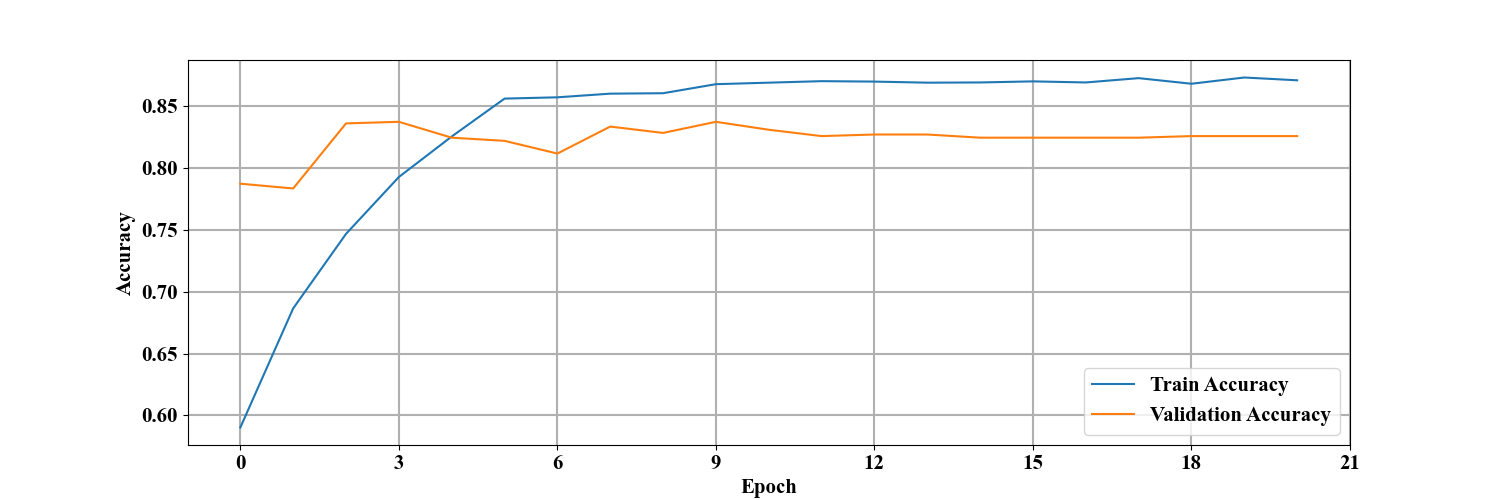
\includegraphics[width=1\linewidth]{images/resultados/sgd_accuracy.png}}
\caption{Acurácia do \acrshort{vit} durante treino e validação.}
\label{fig:acc}
\end{figure}

\begin{figure}[tb]
\centerline{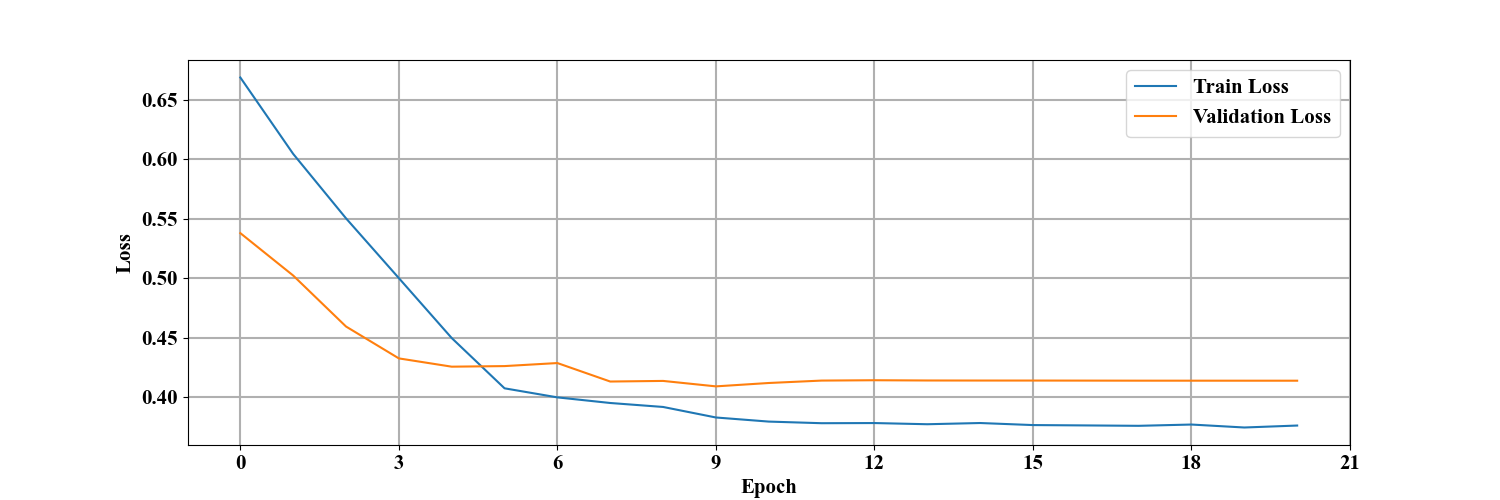
\includegraphics[width=1\linewidth]{images/resultados/sgd_loss.png}}
\caption{Perda do \acrshort{vit} durante treino e validação.}
\label{fig:loss}
\end{figure}

A pequena diferença na acurácia entre os conjuntos de treinamento e validação (Fig. \ref{fig:acc}) pode ser justificada pela introdução de características no conjunto de validação que não estão presentes no conjunto de treinamento.

% ----------------------------------------------------------
\subsection{Melhor modelo com diferentes quantidades de câmeras}\label{sec:cameraquantity}

Com o objetivo de verificar se o aumento da quantidade de câmeras no conjunto de treino levaria a melhorias significativas em sua performance, a arquitetura \acrshort{vit} foi treinada com conjuntos de treino menores.
Esses conjuntos possuem menor quantidade de câmeras, mas mantêm o mesmo número de imagens por classe para cada câmera.

Para compor esses conjuntos comparativos ao utilizado originalmente, dentre as 60 câmeras que compõem o conjunto original, foram escolhidas aleatoriamente 30 câmeras para formar o segundo conjunto.
Dessas 30 câmeras, foram selecionadas aleatoriamente 15 para compor o terceiro conjunto.
Portanto, os três conjuntos de treino possuem as mesmas 15 câmeras, e o conjunto com 60 câmeras inclui todo o conjunto das 30 câmeras, acrescido de outras 30 câmeras adicionais.

Dessa forma, o efeito de adicionar novas câmeras ao conjunto de treino pode ser mais facilmente compreendido.
A Tabela \ref{tab:trainingimages} apresenta a relação entre o tamanho do conjunto de treino, sua acurácia e o tempo de treinamento.
O modelo foi testado utilizando o mesmo conjunto de teste pertencente ao conjunto de dados original.

\begin{table}[!ht]
\begin{center}
\caption{Acurácia $\times$ tempo de treino $\times$ número de imagens usadas}
\label{tab:trainingimages}
\begin{tabular}{c|cc}
%\hline
\toprule
\textbf{\textbf{Nº de Câmeras}} & \textbf{Acurácia} & \textbf{Tempo (minutos)}\\
%\hline\hline
\midrule
15 &  0,728 & 17\\
30 & 0,804 & 18 \\
60 & 0,826 & 21 \\
%\hline
\bottomrule
\end{tabular}
\end{center}
\end{table}

Como esperado, aumentar a diversidade de câmeras no conjunto de treino e, consequentemente, a quantidade total de imagens de treino, resultou em incremento na acurácia do modelo.
Entretanto, o número de câmeras atualmente utilizado mostra-se adequado, pois a inclusão de mais câmeras não trouxe melhorias significativas no desempenho.
Observou-se que dobrar a quantidade de imagens de treino, passando de 1800 para 3600 — ou seja, de 30 para 60 câmeras no conjunto de treino — representou uma melhoria marginal de apenas 0,022 na acurácia.

% ----------------------------------------------------------

\section{Comparação entre diferentes otimizadores}\label{sec:optimizer}
Apesar de, inicialmente, todos os modelos terem sido treinados utilizando o \acrshort{sgd} como otimizador, a escolha de diferentes otimizadores e taxas de aprendizagem pode influenciar significativamente a performance das \acrshort{cnn}.

Com base nos resultados apresentados por Dogo \textit{et al.} \cite{Dogo2022optimizers}, que compararam diversos otimizadores em redes neurais e conjuntos de dados de diferentes tamanhos e complexidades, esta dissertação realizou uma comparação dos resultados do \acrshort{vit} utilizando o \acrshort{sgd}, o \acrlong{adam} \cite{adam} e o \acrlong{nadam} \cite{nadam}.
Todos os otimizadores foram configurados conforme descrito na Seção \ref{sec:methodology_models}, sendo testados com diferentes taxas de aprendizagem iniciais.

\begin{table}[tb]
%\resizebox{\columnwidth}{!}{%
\caption{\label{tab:optimizer_acc} Acurácia do \acrshort{vit} com diferentes otimizadores.}
\begin{center}
\begin{tabular}{c| c c c }
\toprule
\multirow{2}{*}{\begin{tabular}[c]{@{}c@{}}Taxa de \\ Aprendizado\end{tabular}} & \multicolumn{3}{c}{Acurácia}   \\
                                                                                & SGD      & Adam     & NAdam    \\
\midrule
1x10-06                                                                           & 0,504   & 0,833 & 0,819 \\
1x10-05                                                                           & 0,512 & 0,841 & \textbf{0,862} \\
1x10-04                                                                           & 0,826 & 0,636 & 0,650    \\
\bottomrule
\end{tabular}
\end{center}%
%}
\end{table}

\begin{figure}[tb]
\centerline{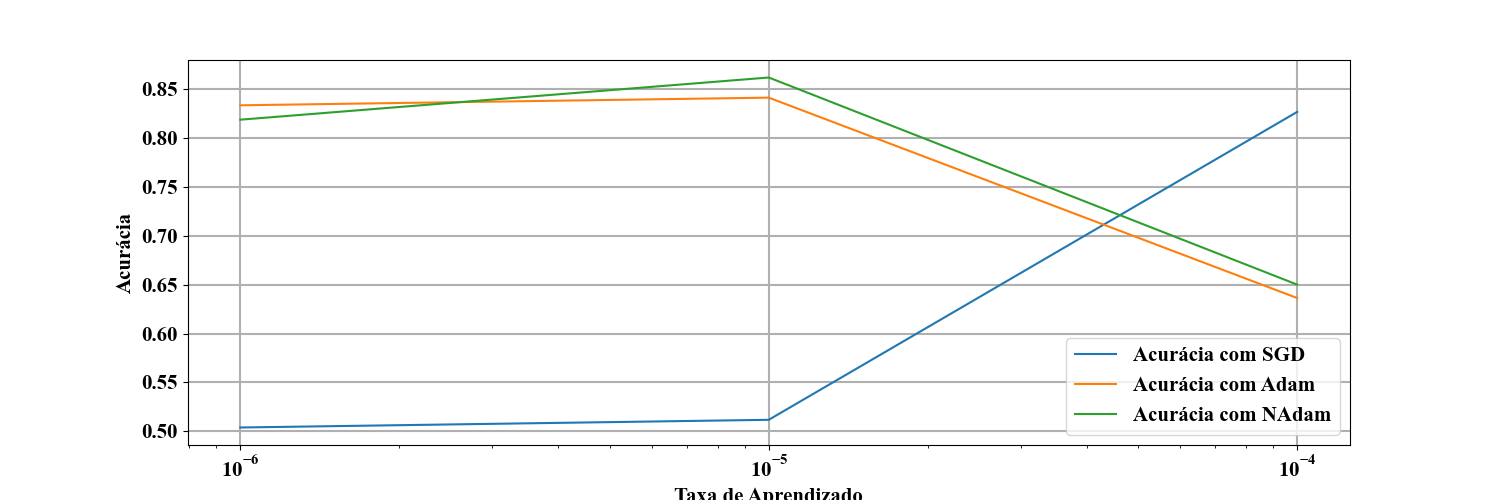
\includegraphics[width=1\linewidth]{images/resultados/optimizer_acc.png}}
\caption{Acurácia do \acrshort{vit} com diferentes otimizadores.}
\label{fig:optmizer_acc}
\end{figure}

Os resultados apresentados na Tabela \ref{tab:optimizer_acc} indicam que tanto o \acrshort{adam} quanto o \acrshort{nadam} apresentaram acurácias superiores ao \acrshort{sgd}.
O \acrshort{nadam} obteve a melhor acurácia, alcançando 0,86 com uma taxa de aprendizado de 1x10$^{-5}$.

Ao analisar o desempenho do \acrshort{sgd}, observa-se que taxas de aprendizado menores resultaram em piores resultados, possivelmente indicando que o passo de atualização foi muito pequeno para escapar de mínimos locais, especialmente em arquiteturas mais complexas, como o \acrshort{vit}.

Nenhum dos otimizadores conseguiu obter um bom desempenho com a menor taxa de aprendizado, o que pode ser explicado pelo fato de que o modelo não realizou atualizações significativas nos pesos durante o treinamento.
As variantes do \acrshort{adam} apresentaram melhor performance com taxas de aprendizado moderadas, com o \acrshort{nadam} se destacando.
A utilização da aceleração de Nesterov para atualizações mais rápidas no \acrshort{nadam} pode ser a principal responsável por seu desempenho superior.

As Figuras \ref{fig:nadam_acc} e \ref{fig:nadam_loss} ilustram a acurácia e a perda do \acrshort{vit} durante o treinamento com o \acrshort{nadam}, utilizando a taxa de aprendizado de 1x10$^{-5}$, momento em que foi obtida a maior acurácia de validação.
Considerando que o modelo estabilizou sua acurácia de treinamento em 1 , enquanto a acurácia de validação se manteve em torno de 0,862, observa-se que o modelo não conseguiu generalizar adequadamente, indicando a ocorrência de \textit{overfitting}.
Esse fenômeno é corroborado pela curva de perda, na qual a perda de validação aumentou, em contraste com a perda de treinamento, que diminuiu para valores próximos a zero.

\begin{figure}[tb]
\centerline{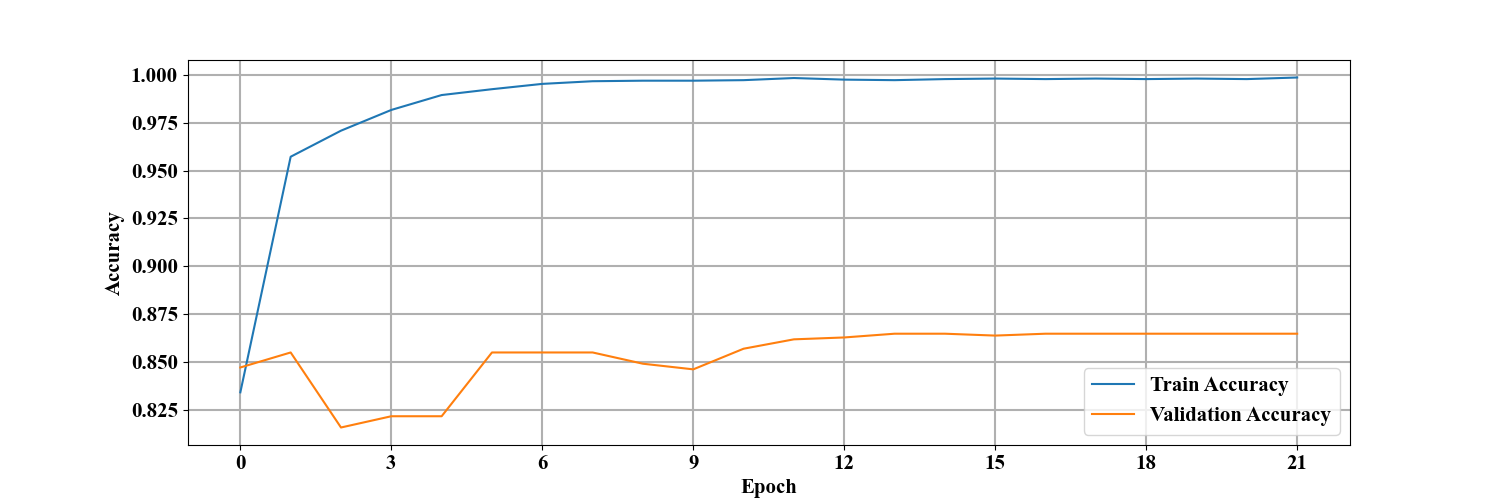
\includegraphics[width=1\linewidth]{images/resultados/nadam_accuracy.png}}
\caption{Acurácia do \acrshort{vit} com NAdam.}
\label{fig:nadam_acc}
\end{figure}

\begin{figure}[tb]
\centerline{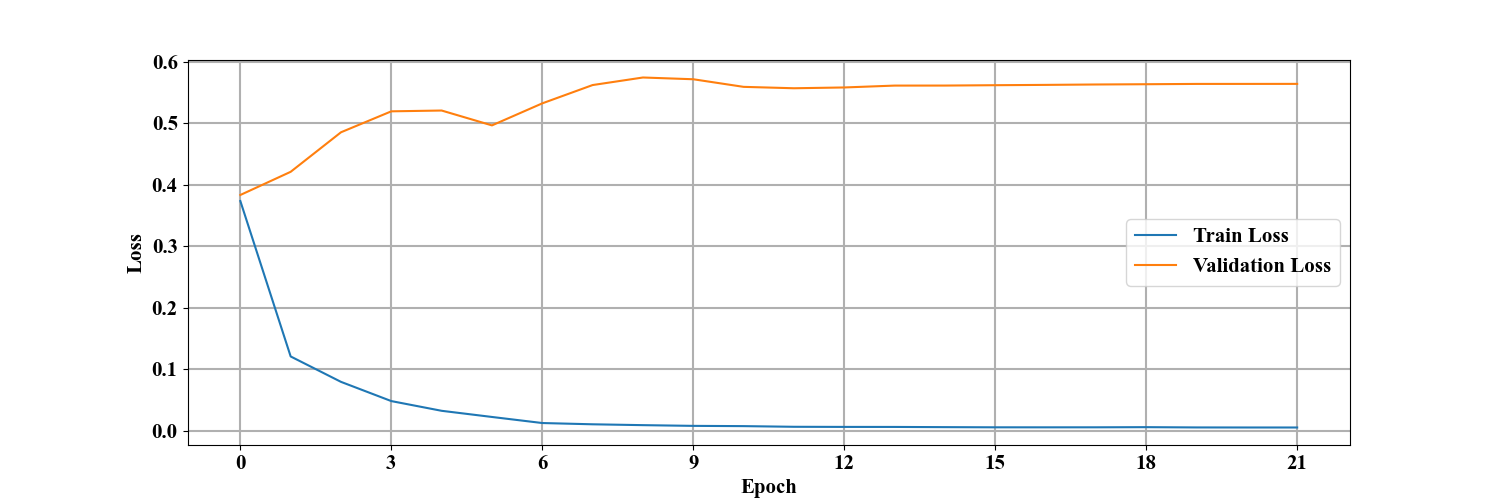
\includegraphics[width=1\linewidth]{images/resultados/nadam_loss.png}}
\caption{Perda do \acrshort{vit} com NAdam.}
\label{fig:nadam_loss}
\end{figure}

Fazendo a mesma análise para a taxa de aprendizagem de 1x10$^{-6}$, onde a acurácia de validação foi um pouco menor, pode-se notar algumas semelhanças e diferenças.
Ainda houve uma diferença significativa entre as acurácias de treino e validação, com a acurácia de treino estabilizando em torno de 0,984, enquanto a acurácia de validação ficou em aproximadamente 0,832.

Entretanto, a curva de perda apresentou melhorias.
Tanto a curva de treino quanto a curva de validação tenderam a diminuir, embora a redução da perda na validação não tenha sido tão significativa.
Este modelo não apresentou sinais claros de \textit{overfitting} como o modelo com maior taxa de aprendizagem, mas ainda demonstra potencial para melhorias.

\begin{figure}[tb]
     \centerline{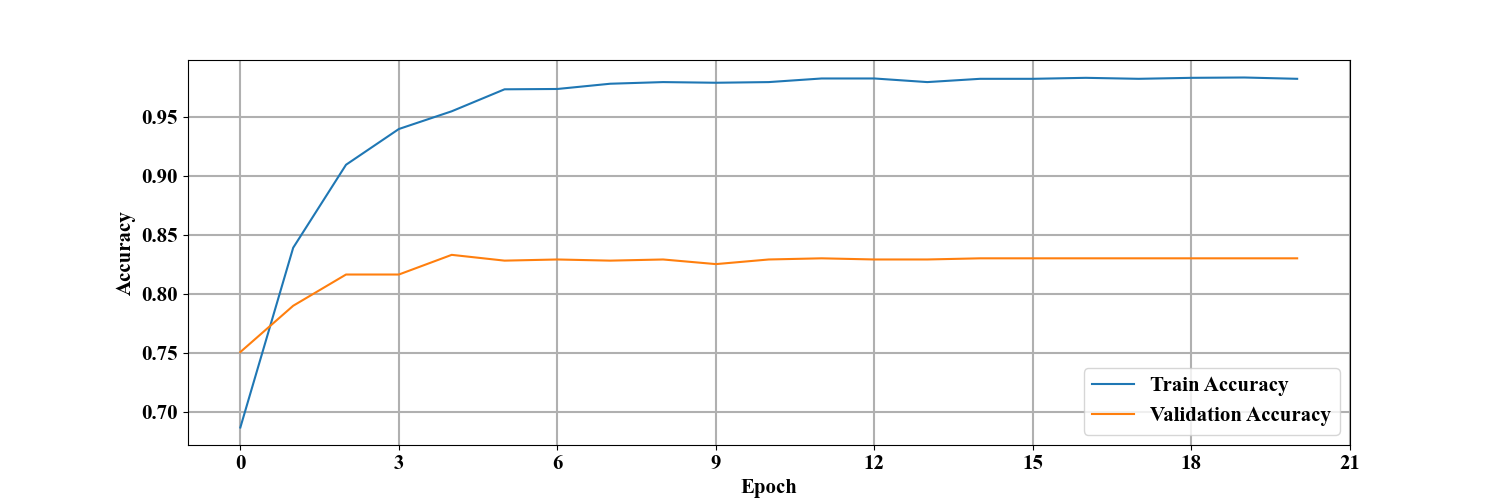
\includegraphics[width=1\linewidth]{images/resultados/nadam_accuracy_1e06.png}}
     \caption{Acurácia do \acrshort{vit} com NAdam e menor taxa de aprendizagem.}
     \label{fig:nadam_acc_1x1006}
\end{figure}
     
\begin{figure}[tb]
     \centerline{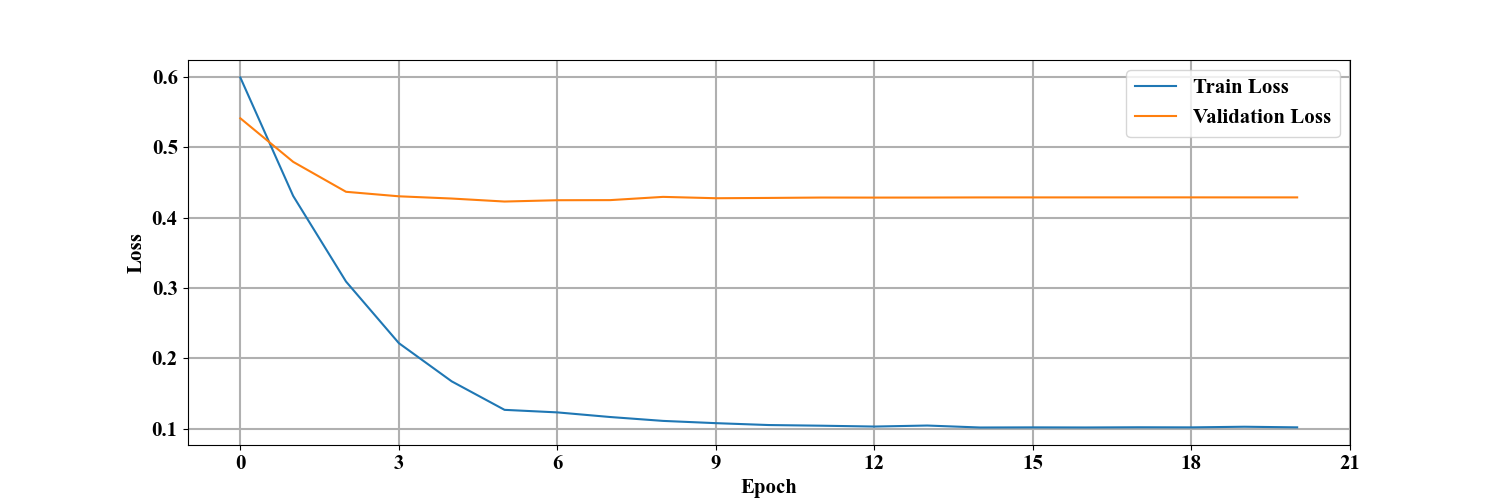
\includegraphics[width=1\linewidth]{images/resultados/nadam_loss_1e06.png}}
     \caption{Perda do \acrshort{vit} com NAdam e menor taxa de aprendizagem.}
     \label{fig:nadam_loss_1x1006}
\end{figure}

Visto que o modelo \acrshort{vit} usando \acrshort{nadam} e taxa de aprendizagem de 1x10$^{-6}$ obteve acurácia de validação semelhante a do modelo com o \acrshort{sgd} de taxa de aprendizagem de 1x10$^{-4}$,
entretanto, teve maior diferença entre as acurácias de treino e validação, assim como redução na função de perda, o modelo com \acrshort{sgd} vai continuar a ser analisado como o melhor modelo, por possuir maior estabilidade.

% ----------------------------------------------------------
\section{Comparações entre cena diurna e noturna}

Para melhor compreender o efeito da iluminação da cena nos resultados de classificação do modelo \cite{piedad2022},
o melhor desempenho do \acrshort{vit} com o otimizador \acrshort{sgd}, descrito na Seção \ref{sec:optimizer}, foi avaliado separadamente em relação às suas métricas para imagens capturadas durante o dia e durante a noite no local.
Os resultados dessa avaliação estão apresentados na Tabela \ref{tab:daynight_acc}.

\begin{table}[tb]
%\resizebox{\columnwidth}{!}
\end{center}
\end{table}

Em contraste com os resultados apresentados e discutidos no Capítulo \ref{cap:trabalhos}, nos quais o modelo exibiu desempenho substancialmente superior em imagens diurnas quando comparado às imagens noturnas \cite{piedad2022},
o modelo treinado com o conjunto de dados \acrshort{rfd} demonstrou diferenças menores na acurácia entre imagens capturadas em condições diurnas e noturnas.
Essa maior estabilidade na acurácia pode ser atribuída à redução da claridade das imagens, obtida por meio do pré-processamento aplicado.

% ----------------------------------------------------------
\section{Outros conjuntos de dados}\label{sec:resultados_outros}

O modelo \acrshort{vit} treinado no conjunto \acrshort{rfd} também foi avaliado em dois outros conjuntos de dados,
o \acrfull{efd} \cite{BarzSchroeterMuench2018_1000117723} e o conjunto de dados de Sazara \textit{et al.} \cite{sazara2019}.
O \acrshort{efd} é composto por 327 imagens da classe normalidade e 252 imagens da classe alagamento, totalizando 579 imagens.
Já o conjunto de dados de Sazara \textit{et al.} contém 491 imagens, das quais 238 correspondem à classe normalidade e 253 à classe alagamento.

Observa-se, na Tabela \ref{tab:vitperformance}, que o desempenho do modelo diminuiu ao ser testado nestes conjuntos distintos.
Apesar do aumento na precisão, houve uma queda significativa na acurácia, indicando que o modelo não conseguiu generalizar adequadamente para imagens com diferentes ângulos, qualidade e condições de iluminação.

\begin{table}[tb]
\caption{\label{tab:vitperformance} Performance do \acrshort{vit} em outros conjuntos de dados}
\begin{center}
\begin{tabular}{c|cccc}
\toprule
 Conjunto de Dados & Acurácia & Precisão & Revocação \\
\midrule
     \acrshort{rfd} & 0,826 & 0,863 & 0,778 \\
     EFD & 0,731 & 0,892 & 0,714 \\
     Sazara & 0,744 & 0,903 & 0,674 \\
\bottomrule
\end{tabular}
\end{center}
\end{table}